\begin{appendices}
\chapter{External Materials}

The project made use of the following external libraries, tutorials and documentation to achieve the end result. The Respective URLs were shortened for brevity but these can be found in fullest at the footnote of the page.

\begin{itemize}
  \item MobileNet-SSD model \url{https://bit.ly/2Hq8yeh}\footnote{\url{https://github.com/chuanqi305/MobileNet-SSD}}. The GitHub repository made available the serialised MobileNet-SSD model used for the detection task. 
  \item Object detection with deep learning and OpenCV \url{https://bit.ly/2vCzTIx}\footnote{\url{https://www.pyimagesearch.com/2017/09/11/object-detection-with-deep-learning-and-opencv/}}. This tutorial provided the insights on how to use the serialised Caffe model and the initial scaffolding code, which was modified for the project's purpose.
  \item Baxter Cashier Robot wiki \url{https://bit.ly/2Hm6eZF}\footnote{\url{https://github.com/papallas/baxter_cashier/wiki}}. The repository's wiki offered a great insight on how to keep the project documented.
  \item Human-Robot Interaction for Cashier Robot \url{https://bit.ly/2vBRwID}\footnote{\url{https://minerva.leeds.ac.uk/bbcswebdav/orgs/SCH_Computing/FYProj/reports/1617/PAPALLAS17-FPR.pdf}}. Rafael Papallas' report was a source of inspiration during the report writing.
  \item Other libraries used include ROS\footnote{\url{http://www.ros.org/}} and OpenCV\footnote{\url{https://opencv.org/}}.
\end{itemize}

\chapter{Legal, ethical, social and professional issues}

\textbf{Privacy Issues}

One of the burning ethical issues is surely the privacy of the data that autonomous system can easily collect within their environment and ultimately process locally or on the cloud. Therefore appropriate consent should be asked beforehand or make the whole estimation process clearer to the people around that data acquisition is in process. The current project's implementation stores people's pictures locally for the person detection process, hence appropriate image consent was asked and submitted as a deliverable. Both the image consent form and information are available in Appendix E and F. 

\textbf{Unemployment and Wealth redistribution}

Unemployment is another issue that sooner or later has to be tackled, as robots become more capable of doing predictable and unpredictable tasks there is a high risk of people loosing their jobs in different areas including care, servicing and logistics. This project is not necessarily involved in any of these sectors, nonetheless, such a professional issue should be taken into consideration.

Wealth redistribution is another pressing topic. How shall the income brought by these robots be managed, should a part of it be given back to the people that lost their jobs to the hands of these autonomous and efficient systems or not.

\chapter{Access To Deliverables}

This appendix lists the web links to some of the project's deliverables. URLs were shortened for brevity but the full ones can be found at the footnote of the page.

\begin{enumerate}
  \item Project's repository: \url{https://bit.ly/2r7ks6k}\footnote{\url{https://github.com/itaouil/human_position_estimation}}
  \item Project's wiki: \url{https://bit.ly/2HAma6t}\footnote{\url{https://github.com/itaouil/human_position_estimation/wiki}}
\end{enumerate}

\chapter{Gantt Chart}

The Gantt chart showing the project progress can be found below. The tasks reflect sprint set in accordance with the weekly meetings had with the project's supervisor. However, these sometimes were completed before the end of the sprint or exceeded the sprint time, hence why there is such a difference in the approximate timing breakdown. The December-January gap is due to exam preparation, where the project was put on hold.

\begin{landscape}
            \newcounter{myWeekNum}
            \stepcounter{myWeekNum}

            \newcommand{\myWeek}{
                \themyWeekNum
                \stepcounter{myWeekNum}
                \ifnum\themyWeekNum=04
                    \setcounter{myWeekNum}{1}
                \else\fi
            }

            \setcounter{myWeekNum}{04}
                \ganttset{
                calendar week text={\myWeek{}}
            }

            \begin{ganttchart}[
                x unit=.9mm,
                hgrid style/.style={draw=black!5, line width=.75pt},
                vgrid={*{6}{draw=none},dotted},
                y unit title=.6cm,
                y unit chart=.6cm,
                time slot format=isodate,
                time slot format/start date=2017-10-01]{2017-10-01}{2018-04-30}
                \ganttset{bar height=.8}
                \gantttitlecalendar{year, month} \\
                    \ganttgroup{\textbf{Phase 1}}{2017-10-01}{2017-12-16}\\
                        \ganttbar{Background \& Research}{2017-10-01}{2017-11-01}\\
                        \ganttbar{Develop basic detection module}{2017-11-01}{2017-11-15}\\
                        \ganttbar{Extend module to run on ROS}{2017-11-16}{2017-11-21}\\
                        \ganttbar{Develop conversion module}{2017-11-22}{2017-11-30}\\
                        \ganttbar{Create custom detections messages}{2017-12-01}{2017-12-05}\\
                        \ganttbar{Test basic detection on TIAGO}{2017-12-06}{2017-12-16} \ganttnewline

                    \ganttgroup{\textbf{Phase 2}}{2018-01-22}{2018-03-15}\\
                        \ganttbar{Develop basic distance module}{2018-01-22}{2018-02-14}\\
                        \ganttbar{Integrate ROS services as paradigm}{2018-02-15}{2018-02-22}\\
                        \ganttbar{Solve distance bugs}{2018-02-22}{2018-02-28}\\
                        \ganttbar{Create custom distance messages}{2018-03-01}{2018-03-05}\\
                        \ganttbar{Prepare presentation}{2018-03-06}{2018-03-10}\\
                        \ganttbar{Test intermediate solution on TIAGO}{2018-03-11}{2018-03-15} \ganttnewline

                    \ganttgroup{\textbf{Phase 3}}{2018-03-17}{2018-04-30}\\
                        \ganttbar{Extend distance module to compute 3D pose}{2018-03-17}{2018-03-31}\\
                        \ganttbar{Create visual markers for RVIZ}{2018-04-1}{2018-04-6}\\
                        \ganttbar{Testing \& Evaluation}{2018-04-7}{2018-04-23}\\

                    \ganttgroup{------------}{2017-10-01}{2018-04-30}\\
                        \ganttbar{Report Writing}{2017-10-01}{2018-04-30}\\
                        \ganttmilestone{Project Submission}{2018-04-30} \ganttnewline
            \end{ganttchart}
        \end{landscape}

\chapter{Image Consent Information}

\begin{figure}[H]
  \begin{center}
    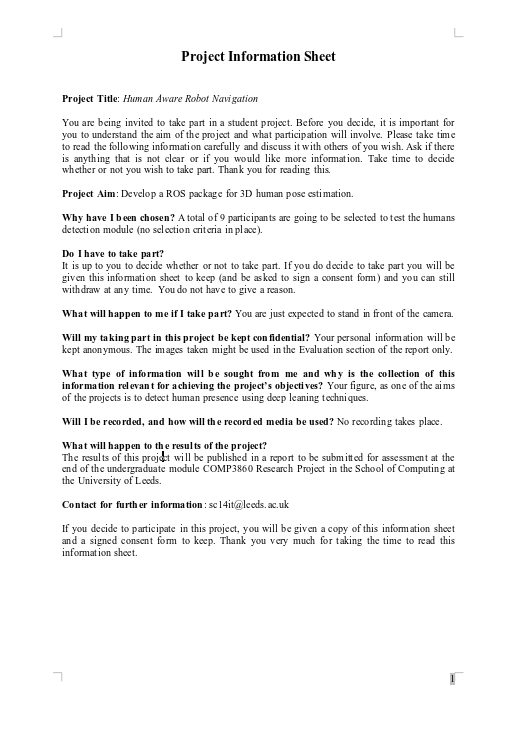
\includegraphics[width=.9\linewidth]{images/appendix_consent_info.png}
  \end{center}
\end{figure}

\chapter{Image Consent Form}

\begin{figure}[H]
  \begin{center}
    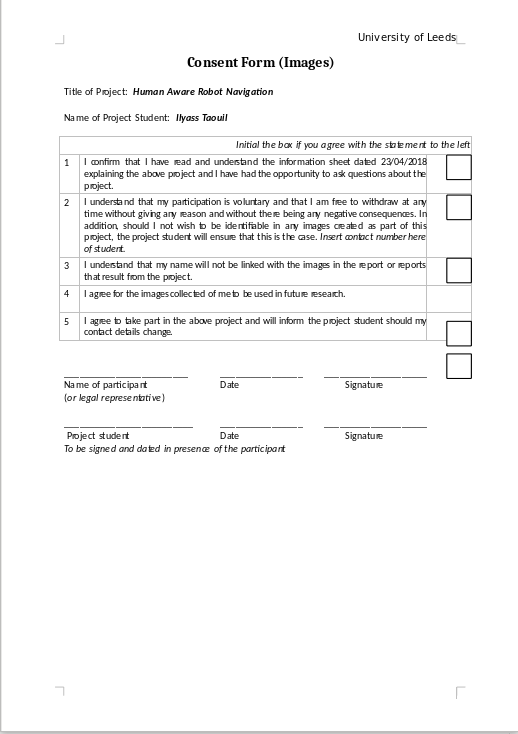
\includegraphics[width=.9\linewidth]{images/appendix_consent_form.png}
  \end{center}
\end{figure}

\end{appendices}